% http://www.math-linux.com/spip.php?article77 <<-- hyvää referenssipikkutietoa
% Abs {{{
\documentclass[]{beamer}
\usepackage[orientation=landscape,size=custom,width=16,height=9,scale=0.5,debug]{beamerposter} 
\usepackage[utf8]{inputenc}
\usepackage[finnish]{babel}
\usepackage[T1]{fontenc}

%\usepackage{handoutWithNotes}
%\pgfpagesuselayout{4 on 1 with notes}[a4paper,border shrink=5mm]

\setbeamertemplate{background canvas}[vertical shading][bottom=blue!20,top=cyan!20]
\usepackage {graphicx}
\graphicspath { {./kuvat/} } 

% pari komentoa
% graafisiin ohjelmiin viittailu
\newcommand{\Gohj}[1]{\emph{#1}}
% tekstiohjelmiin ja komentoihin viittailu
\newcommand{\Tohj}[1]{\texttt{#1}}
\newcommand{\com}[1]{{\color{blue!50!black}\Tohj{#1}} \!\!}

% vim-asetuksiin viittailu
\newcommand{\set}[1]{\texttt{#1}}
\newcommand{\code}[1]{\texttt{#1}}
\newcommand{\key}[1]{\texttt{#1}}

% värittelykomentoja taulukkoa varten
% LaTeXissa soisi tulevan tätä varten lokaalit määrittelyt, myös esittelyosan jälkeen
\newcommand{\Move}[1]{{\color{red}#1}}
\newcommand{\Insert}[1]{{\color{green}#1}}
\newcommand{\Modify}[1]{{\color{purple}#1}}

\AtBeginPart
{
    \frame {
        \frametitle{Osa \insertpartnumber : \insertpart}
        \tableofcontents
    } 
}

\AtBeginSection[]
{
    \begin{frame}
        \tableofcontents[currentsection]
    \end{frame}
}


\title[Vim]{Vi Improved}
\author{M. Puhakka}
\date{\today}


% }}}
\begin{document}
% Osa 1: Perusteet {{{

\part {Esittely ja perusteet}

\section{Editorit}
\begin{frame}
    \frametitle{Editori, mitä ne ovat?}
    \begin{itemize}
        \item Editori on työvälineohjelma, jolla muokataan ja kirjoitetaan puhdasta tekstiä.
        \pause
        \item Esimerkiksi Windowsin \Gohj{Muistio}, maksullinen \Gohj{UltraEdit} ja DOSin \Tohj{Edit}. 
        \item  \Gohj{Microsoft Word} ei ole editori, vaan tekstinkäsittelyohjelma.
    \end{itemize}
\end{frame}

\begin{frame}[plain]
  \includegraphics[width=\textwidth]{ultraedit-32-16752-1}
\end{frame}

\begin{frame}
  \frametitle{Mihin editoreja käytetään?}
  \begin{itemize}
    \item Tekstimuotoinen data on pääasiallinen käyttökohde. Kuitenkin myös isommat ohjelmakokonaisuudet sisältävät pienimuotoisempia editoreja
    \item Käytännössä esimerkiksi \Gohj{Word} koostuu editorista, asetteluohjelmasta, kielioppitarkistimesta, \ldots
    \pause
    \item Vanhaan hyvään aikaan editori oli työmiehen ainut työkalu. Sen parissa kirjoitettiin koodi, tehtiin raportit ja viimeisteltiin työpäiväkirja.
    \item Editorin virittelyyn ja hienosäätöön kulutettiin aikaa, koska monissa tapauksissa koko työpäivän kaikki näyttöpäätetyöskentely tehtiin yhden ohjelman sisällä, editorin.
  \end{itemize}
\end{frame}

\begin{frame}[plain]
  \includegraphics[width=\textwidth]{notepad2}
\end{frame}

\section{Editorien evoluutio}

\begin{frame}
  \frametitle{Editorien ajanlaskun alussa: rivieditorit}
  \begin{itemize}
    \item Kun näyttötila oli kallista, ulkoverkkoja ei ollutkaan ja silti näppäimistöpainallusta seurasi sekuntien viive, oli monesti tehokkainta käyttää sellaista editoria, joka ei turhia räikeile hienouksilla
    \pause
    \item \ldots hienouksilla, kuten esimerkiksi asiakirjan teksti. Tiedostosta luettiin pyytämällä rivejä lyhyillä kryptisillä komennoilla kuten \code{2p} ja sinne lisättiin tekstiä vaikkapa komentojen kuten \code{5i} tapaan.
    \note {Ed, Edlin}
\end{itemize}
\end{frame}

\begin{frame}[t]
\frametitle{Unix-ajan vörmyt}

Kultaisella 70- ja 80-luvulla Unix-mainframeilla työskennelleillä oli valittavanaan kahdenlaista editoria, joista kumpikin edusti omanlaista suunnittelufilosofiaansa.

\vspace{0.4cm}
\begin{columns}[t]
 \begin{column}{0.5\textwidth}
  \textbf{Vi}
  \begin{itemize}
    \item Kevyt
    \item Vain tärkeimmät perustoiminnot
    \item Nopeille kirjailijoille
    \end{itemize}
\end{column}
\begin{column}{0.5\textwidth}
  \textbf{Emacs}
  \begin{itemize}
    \item Raskas
    \item Monipuolinen
    \item Todella monipuolinen
    \end{itemize}
\end{column}
\end{columns}
\vspace{0.4cm}

Me keskitymme nyt tässä tämän editorikatsauksen toiseen osapuoleen, \Tohj{Vi}:hin, ja erityisesti sen kehittyneeseen nykyversioon.
\end{frame} 

\begin{frame}
  \frametitle{Palanen Emacsia}
  \includegraphics[width=\textwidth]{27-04_emacs}
\end{frame}

\begin{frame}[plain]
    \frametitle{Vi ja Emacs}
    Nämä kaksi ovat olleet keskenään ''sodassa'' aina 70-luvulta lähtien. Nykypäivän graafinen sukupolvi ei enää näytä välittävän aiheesta tarpeeksi lietsotakseen sanasotaa.

    \includegraphics[width=\textwidth]{0010_en_vi-vs-emacs}
\end{frame}

\section{Vim}

\begin{frame}
  \frametitle{Vim tämän työn kimpussa}
  \includegraphics[width=\textwidth]{gvim}
\end{frame}

\begin{frame}
\frametitle{Mikä tekee Vi:stä erikoisen?}
\begin{itemize}
    \item Lyhyesti sanottuna: sen modaalisuus
    \item Toimintavarmuus ja keveys olivat alkuperäisen Vi:n toiset vahvuudet
    \item \ldots ja sen jatkaja Vim lisäsi joukkoon laajennettavuuden ja monipuolisuuden
    \pause
    \item Alkuperäinen Vi muodostaa ydintoiminnallisuuden, jonka parissa nyky-Viminkin parissa työskennellään 90\% ajasta, vaikka ne käsittävätkin vain 10\% kaikista Vimin toiminnoista
\end{itemize}
\end{frame}

\begin{frame}
    \frametitle{Modaalisuus, mitä?}
    \begin{itemize}
        \item Vi koostuu kahdesta pääasiallisesta toimintamoodista: normaali- ja lisäysmoodista
        \pause
        \begin{itemize}
            \item <+-| alert@+> normaalimoodissa liikutaan asiakirjassa erilaisten näppäinten avulla
            \item <+-| alert@+> lisäysmoodissa lisätään uutta tekstiä haluttuun kohtaan. Puhdasoppiset vi-käyttäjät eivät tee liikettäkään normaalimoodin ulkopuolella, vaikka se olisikin mahdollista
        \end{itemize}
        \pause
        \item Koska kovin harva massojen suosima editori käyttää enää modaalisuutta, on se taiteenlaji redusoitunut lähinnä tänne vi-maailmaan. 
        \pause
        \item Modaalisuuden edut ovat kuitenkin selvät verrattuna de facto -standardiksi ajateltavaan \emph{modifier}-malliin
    \end{itemize}
\end{frame}


\section {Vi:n perusasiat}

\begin{frame}
    \frametitle{Tekstissä liikkuminen 1}
    \begin{columns}
    \begin{column}{0.8\textwidth}
    \begin{itemize}
        \item Jo pitkään käytetty nuolinäppäimistö on itse asiassa hyvin epäergonominen
        \item Vi käyttää ergonomisia näppäimiä normaalimoodissa, joilla tehdään perusliikkumista tekstissä
        \item Vaikka nykyisin voi käyttää nuolinäppäimiäkin liikehdintään, on hyvä edes kokeilla (ja huomata HJKL paljon mukavammaksi) vaihtoehtoista systeemiä
    \end{itemize}
    \end{column}
    \begin{column}{0.2\textwidth}
        \includegraphics[width=\textwidth]{hjkl}
    \end{column}
    \end{columns}
\end{frame}

\begin{frame}
    \frametitle{Käynnistys ja lopetus}
    \begin{itemize}
        \item Käynnistys: Unix-piireissä komennolla \code{vi [tiedosto.tex]}, Windowseissa tyypillisesti klikkaillaan kuvakkeesta
        \item Sammutus: normaalimoodissa yleisin tapa on \com{:q} (lyh. quit) 
        \item Avaus: normaalimoodissa \com{:e} (lyh. edit) avaa tiedoston. Nimeä on osattava tavata, tai voi käyttää tekstigraafista selausohjelmaa. Windowsissa standardi avausdialogi
        \item Tallennus: normaalimoodissa \com{:w} (lyh. write). Tallenna ja lopeta: joko \com{:wq} tai ytimekkäämpi \com{:x} tahi \key{ZZ} (kaksi kertaa iso Z-kirjain)
    \end{itemize}
\end{frame}

\section{Tekstinkäsittely}

\begin{frame}
    \frametitle{Tekstin kirjoittaminen}
    \begin{itemize} 
        \item Editorin yleisin tehtävä; vi tarjoaa kymmeniä tapoja lisäillä tekstiä.
        \item Lisäysvaiheessa siirrytään normaalimoodista lisäysmoodiin: näppäimet (kuten h, j, k, l) tuottavatkin nyt kirjaimia näytölle ''kuten pitäisikin''
        \pause
        \item Kun valmista, palataan normaalitilaan painamalla \com{<Esc>}
        \pause
        \item Keskeinen lisäyskomento \com{i} (lyh. insert): aloittaa tekstin lisäämisen täsmälleen kursorin kohdalle
        \item Samanhenkinen komento on \com{a} (lyh. append): vastaa samaa kuin komento \com{li}
    \end{itemize}
\end{frame}

\begin{frame}
    \frametitle{Tekstissä liikkuminen 2}
    Hyvin perustavat komennot \com{w}, \com{e}, \com{b}, \com{0} ja \com{\$}:
    \includegraphics[width=\textwidth]{vi_liikekomennot_web0}
\end{frame}

\begin{frame}
    \frametitle{Tekstissä liikkuminen 3}
    \begin{itemize}
        \item Edellisen kalvon komennot \com{w}, \com{e} ja \com{b} käyttävät hyväkseen termiä ''sana'', joka tarkoittaa yhtä aakkosnumeerista rykelmää, jonka molemmin puolin on jokin erikoismerkki tai rivin alku/loppu
        \pause 
        \item Tämä voi olla työlästä, jos sanojen seassa on paljon erikoismerkkejä, kuten pilkkuja, kysymysmerkkejä ynnä muuta sellaista
        \pause
    \end{itemize}
        \begin{columns}
        \begin{column}{0.7\textwidth}
            \begin{itemize}
            \item Ratkaisuna on erillinen käsite \emph{''big word''} joka on suomalaisittain helppo omaksua: yhdyssana \emph{linja-auto} koostuu kahdesta pienestä sanasta, ja muodostaa yhden ison sanan
            \item Helppo muistaa: korvaa pieni komento isolla kirjaimella
            \end{itemize}
        \end{column}
        \begin{column}{0.2\textwidth}
            \includegraphics[width=\textwidth] {vi_bigword}
        \end{column}
        \end{columns}
\end{frame}

\begin{frame}
    \frametitle{Tekstin lisäily 2}
    \begin{itemize}
        \item Vaikka käyttämällä komentoa \com{i} joka paikkaan pääseekin hyvin pitkälle, on vimissä tarkoituksella hyvin monia keinoja päästä lisäilemään tekstiä uusiin paikkoihin, kaikki joustavuuden nimissä
        \item Komennot \com{I} ja \com{A}: lisää rivin alkuun ja loppuun tekstiä. Hyvin näppärä.
        \pause
        \item Komennot \com{O} ja \com{o}: tee tyhjä rivi rivin yläpuolelle / alapuolelle ja lisää sinne
    \end{itemize}
\end{frame}

\begin{frame}
    \frametitle{Tekstin poistaminen}
    \begin{itemize}
        \item Tekstin poistaminen on joskus tarpeen. Vim tukee komentoa \com{d} (lyh. delete), joka ottaa kaverikseen \emph{liikkumakomennon}. Liikkumakomennon kursorista hyppykohtaan oleva pala poistetaan
        \item Esimerkkejä: olkoon tekstinä \texttt{Linja-autolla {\color{red}{m}}atkustaminen on mukavaa}. Ja kursori punaisessa kohdassa. Komentamalla \com{dw} poistettaisiin teksti \texttt{matkustaminen}. Komentamalla \com{d0} vastaavasti mennään taaksepäin, ja poistettaisiin teksti ''\texttt{Linja-autolla }''.
        \pause
        \item Koko rivin voi poistaa nopealla oikopolulla \com{dd}.
        \item Teksti palautettavissa joko perumalla \com{u} (lyh. undo) tai liittämällä teksti rekisteristä komennolla \com{p} (lyh. put)
    \end{itemize}
\end{frame}

\begin{frame}
    \frametitle{Tekstin korvaaminen}
    \begin{itemize}
        \item Tekstiä voi korvata muutamalla tavalla. Kaikki korvausmenetelmät ovat oikopolkuja sille, että ensin poistetaan sana ja siirrytään lisäysmoodiin. Kaikki menetelmät ovat hyvin käytettyjä sopivissa paikoissa
        \item Keskeinen komento on {\color<2>{red}{\com{c} (lyh. change)}}, joka ottaa deleten tapaan suunnan komennon jälkeen. Esimerkiksi \com{c2w} poistaisi kursorin edestä kaksi sanaa, ja siirtyisi sitten lisäystilaan.
        \item Komentamalla nopealla oikopolulla {\color<3>{red}{\com{cc} }} tai vaihtoehtoisesti {\color<3>{red}{\com{S} (lyh. substitute)}} korvataan koko nykyinen rivi alusta alkaen
    \end{itemize}
\end{frame}

\begin{frame}
    \frametitle{Pikkukomentoja ja korvauksia}
    \begin{itemize}
        \item Poista yksi merkki kursorin alta: \com{x}
        \pause
        \item Korvaa yksi merkki kursorin kohdalta: \com{r}, jonka jälkeen korvaava merkki:
        \item Esimerkiksi lause \texttt{Linja-a{\color{red}a}to}, näppäily \com{ru} muuttaa sanan oikeinkirjoitetuksi
        \pause
        \item Yksi tyylikäs tapa korvata tekstiä on \com{R}, joka heittää editorin lisäysmoodiin, mutta siten, että lisätty teksti korvaa aiemman. Vastaa tavallisten editorien Insert/Replace -toimintaa
    \end{itemize}
\end{frame}

\begin{frame}
    \frametitle{Vi-komentojen anatomia}
    \begin{itemize}
        \item On olemassa kahdenlaisia komentoja:
        \pause
        \begin{itemize}
            \item Sellaisia, jotka ottavat liikkeen argumentikseen
            \item Sellaisia, jotka eivät ota mitään
        \end{itemize}
        \pause
        \item Lisäksi komennot voivat ottaa numeroarvoja ikään kuin kertoimeksi eteensä.
        \pause
        \item Jos \com{dw} poistaa yhden sanan, simppelisti \com{d3w} poistaakin kolme sanaa. Kerroinluku voi sijaita myös aivan edessä: \com{3dw} $=$ \com{d3w}
        \pause
        \item Yleisesti: jos \emph{\color{red}a} on komento, \emph{\color{blue}m} on liikekomento ja {\color{purple}$n \in \mathbb{N}$} on kerroin, niin kaikki suuntia ottavat vi-komennot toimivat näin: \emph{{\color{red}a} {\color{purple}n} {\color{blue}m}} tai \emph{{\color{purple}n} {\color{red}a} {\color{blue}m}}
    \end{itemize}
\end{frame}

% }}}
% Osa 2: Lisää käsittelyä {{{
\part {Tekstinkäsittelyä}

\section {Pari kehittynyttä liikekomentoa}

\begin{frame}
    \frametitle {Rivillä liikkuminen}
    \begin{itemize}
        \item Hyppääminen rivillä haluttuun merkkiin: \com{f} ja \com{F}, joita seuraa haluttu kirjain.
        \item Vim etsii annettua merkkiä vain senhetkiseltä riviltä. Löydettyään kursori siirtyy sinne
        \pause
        \item Esimerkki: \texttt{{\color<2>{red}L}ause{\color<3-4>{red},} {\color<4>{red}jossa on jotain turhaa välissä,} jatkuu normaalisti}.
        \item Komennetaan \com{{\color<3>{red}f,}{\color<4>{red}df,}}
        \item<5> Tuloksena: \texttt{Lause jatkuu normaalisti.}
    \end{itemize}
\end{frame}

\begin{frame}
    \frametitle {Isompia liikkeitä}
    \begin{itemize}
        \item Olemme oppineet perusliikkeitä, kuten liikehdinnän rivi tai merkki kerrallaan 
        \item Myös hieman mielekkäämpiä komentoja, kuten hyppelyt sanojen välillä hallussa $\to$ vähentää kovasti tarvetta \com{h}:n ja \com{l}:n käyttöön
        \pause 
        \item Siirtyminen virkkeiden välillä: \com{(} ja \com{)}. Vim tunnistaa virkkeet pisteen, huuto- tai kysymysmerkin avulla. Helppo aloittaa vaikka kesken oleva lause alusta komennolla \com{c(}.
        \item Siirtyminen kappaleiden välillä: \com{\{} ja \com{\}}. Tyhjä rivi, tai useampi, tekstirivien välissä toimii kappale-erottimena.
    \end{itemize}
\end{frame}

\begin{frame}
    \frametitle {Isompia liikkeitä 2}
    \begin{itemize}
        \item Ruudulla näkyvässä sisällössäkin on nopeata liikkua kolmella komennolla:
        \item \com{H} (head) -- hyppää ruudun yläreunaan
        \item \com{M} (middle) -- hyppää keskelle ruutua
        \item \com{L} (low) -- hyppää ruudun alareunaan
        \pause
        \item Hyppääminen tiedoston alkuun: \com{gg}
        \item Hyppääminen tiedoston loppuun: \com{G}
        \item Hyppääminen halutulle riville: \com{:\#}, missä \# rivinumero
    \end{itemize}
\end{frame}

\begin{frame}
    \frametitle {Yhteenvetoa keskeisistä komennoista}
    {\color{red}Liikkuma-}, {\color{purple}lisäys-} ja {\color{blue}muokkaus}komentoja:
    \begin{tabular}{lrlrlr}
    \hline
    \color{red}\com{wW} & \color{red}seur. sanan alkuun
        & \color{purple}\com{i}  & \color{purple}Lisää nyk. kohtaan
        & \color{blue}\com{d}  & \color{blue}Poista\footnote{vaatii liikekomennon}\\
    \color{red}\com{bB} & \color{red}nyk. sanan alkuun
        & \color{purple}\com{a}  & \color{purple}Lisää seur. ruutuun
        & \color{blue}\com{dd}  & \color{blue}Poista rivi\\
    \color{red}\com{eE} & \color{red}nyk. sanan loppuun
        & \color{purple}\com{I}  & \color{purple}Lisää rivin alkuun
        & \color{blue}\com{c}  & \color{blue}Korvaa teksti\footnotemark[\value{footnote}]\\
    \color{red}\com{0}  & \color{red}rivin alkuun
        & \color{purple}\com{A}  & \color{purple}Lisää rivin loppuun
        & \color{blue}\com{cc}  & \color{blue}Korvaa rivi\\
    \color{red}\com{\$} & \color{red}rivin loppuun
        & \color{purple}\com{o}  & \color{purple}Avaa uusi rivi alas
        & \color{blue}\com{x}  & \color{blue} Poista merkki\\
    \color{red}\com{gg} & \color{red}tiedoston alkuun
        & \color{purple}\com{O}  & \color{purple}Avaa uusi rivi ylös
        & \color{blue}\com{r}  & \color{blue}Korvaa merkki \\
    \color{red}\com{G} & \color{red}tiedoston loppuun
        & \color{red}\com{fa}  & \color{red}Etene merkkiin $a$
        & \color{blue}\com{R}  & \color{blue}dyn. korvaus \\
    \color{red}\com{:\#} & \color{red}riville $\#$
        & \color{red}\com{Fa}  & \color{red}Peräänny merkkiin $a$ 
        & \color{red}\com{\{}  & \color{red}Edellinen kappale \\
    \color{red}\com{(}  & \color{red}virkkeen alkuun
        & \color{red}\com{)} & \color{red}virkkeen loppuun
        & \color{red}\com{\}} & \color{red}seuraava kappale \\
    \end{tabular}
\end{frame}

\section {Tekstin ''maalaus'' -- visual-moodi}

\begin{frame}
    \frametitle{Visual-moodi}
    \begin{itemize}
        \item Tyypillinen vim-operaatio, vaikkapa tekstin poisto, koskettaa usein isoa tai muuten epämääräistä lohkoa tekstiä
        \item Tämmöistä lohkoa on usein hankala tai mahdotontakin valita järkevästi \emph{yhdellä} liikekomennolla, vaan liikkeitä tarvitaan useampia
        \pause
        \item Ratkaisuna on visual-moodi! Moodiin pääsee painamalla \com{v}, ja sen jälkeen käytetäänkin tavallisia liikekomentoja aivan tavalliseen tapaan
        \item Teksti maalautuu komentojen mukana, joten ihmisen on helppo havaita, mitä ollaan valitsemassa. Toiminta näyttää aivan kuin graafisten ohjelmien kanssa hiirellä maalaillessa tekstiä
    \end{itemize}
\end{frame}

\begin{frame}
    \frametitle{Visual-moodi 2}
    \begin{itemize}
        \item Siinä missä tavallinen \emph{komento-kerroin-liike} toimii ilman visual-moodia, tarvitaan nyt hieman toisenlainen lähestymistapa
        \item Visual-moodissa ensin valitaan alue, sitten sille jokin komento, usein pelkkä \com{d} tai \com{c}. Visual-moodin valintojen kanssa voi käyttää myös erikoisia komentoja, kuten vaikkapa \com{r}:ää.
        \pause \item
        \begin{enumerate}
            \item \com{v}: visualize
            \item liiku ja valitse haluamasi alue
            \item aseta maalatulle alueelle komento
        \end{enumerate}
    \end{itemize}
\end{frame}

\begin{frame}
    \frametitle{Visual-moodi 3}
    \begin{itemize}
        \item Pikku-\com{v}een lisäksi joissain tilanteissa näppärä visual-moodin erikoistapaus on iso \com{V}, riveittäinen valinta
        \item Käytännössä parin rivin valinta käyttäen (toivottavasti) selkäytimestä tulevilla näppäimillä \com{j} ja \com{k}, \com{V} on hyvin nopea verrattuna \com{v}:hen.
        \pause
        \item Esimerkki: muunna rivi tekstiä -- kaikki kirjaimet pisteiksi:
        \item \com{Vr.} tekee homman: \com{V} valitsee oletuksena jo aktiivisen rivin kokonaan, se riittää. Komento \com{r} toimii visuaalimoodin kanssa siten, että se käy jokaisen merkin läpi, ja muuntaa sen tässä tapauksessa pisteeksi ''.''.
    \end{itemize}
\end{frame}

% text objects!

\begin{frame}
    \frametitle{Tekstiobjektit}
    \begin{itemize}
        \item Visual-moodissa voi valita tekstiä muillakin tavoilla kuin vain liikehtimällä tuttujen komentojen avulla. Tässä moodissa on määritelty joitain näppäimiä uusiksi tarjoten varsin sulavaa joustavuutta askareita varten
        \pause
        \item Esimerkki: \com{vap}: \emph{visualize a paragraph}, valitsee koko kappaleen, sekä sitä seuraavan tyhjän rivin. Komentamalla \com{vapd} poistetaan se kappale, jonka sisällä kursori sattuu olemaan.
        \pause
        \item Tekstiobjekteja voi joissain paikoissa käyttää myös ilman visual-moodia: edellinen komento sujuisi myös näin: \com{dap}: \emph{delete a paragraph}
    \end{itemize}
\end{frame}

\begin{frame}
    \frametitle{Tekstiobjektit 2}
    \begin{itemize}
        \item Tekstiobjekteja on monenlaisia, mutta jokaista niitä yhdistää alkukirjain \com{a} (engl. a) tai \com{i} (engl. inner)
        \item ero on hiuksenhieno: \com{i} jättää mahdolliset välit rauhaan. Kappaleiden tapauksessa tyhjät rivit, lauseiden tapauksessa välit.
    \end{itemize}
\end{frame}

\begin{frame}
    \frametitle{Tekstiobjektit 3}
    Mitä objekteja on sitten käytettävissä? Tehdään lyhyt listaus käytetyimpiin. \\
    \vspace{0.4cm}
    \begin{tabular}{lrr}
    \hline
    kirjain & a:n kanssa & i:n kanssa \\
    {\color{red}{$x$}} & a{{\color{red}{$x$}} } & i{\color{red}{$x$}} \\
    \hline \hline
    \com{w/W} & sana/isosana ja sitä seuraava väli & pelkkä sana\\
    \com{p} & kappale + tyhjä rivi & pelkkä kappale\\
    \com{s} & virke + väli & pelkkä virke \\
    \com{(} tai \com{)} & sulut sisältöineen & pelkkä sisältö \\
    \com{''}, \com{'} tai \com{`} & ``lainatun tekstin'' valinta hipsuineen & pelkkä sisältö\\
    \end{tabular}
\end{frame}

\section {Rekisterit -- Vimin vastine leikepöydälle}

\begin{frame}
    \frametitle{Perusleikepöytäily}
    \begin{itemize}
        \item Keskeiset komennot ovat yhtä helppoja omaksua kuin graafisissa ohjelmissakin:
        \item \com{d}: \emph{delete}, joka toimii samalla myös leikkaustoimintona
        \item \com{y}: \emph{yank}, kopioi poistamatta tekstiä
        \item \com{p}: \emph{put} tai \emph{paste}. Liittää tekstin alkaen kursoria seuraavasta ruudusta
        \item \com{P}: kuten edellä, mutta liittää tekstin alkaen juuri senhetkisestä ruudusta
    \end{itemize}
\end{frame}

\begin{frame}
    \frametitle{Rekisterit ovat vimin leikepöytä}
    \begin{itemize}
        \item Vimissä on 27 rekisteriä käyttäjän omille teksteille, joihin voi joko sijoittaa tai lisätä tekstiä tiedostosta. Lisäksi on erikoisrekistereitä, joista ehkä tuonnempana
        \item Rekisteriin viitataan aakkosella, ja merkitään eteen lainausmerkki \com{"}, jota seuraa rekisterin nimi
        \pause
        \item Esimerkiksi haluamme leikata sanan rekisteriin a: \com{\textquotedbl adw}
        \item Nyt tämän sanan voi liittää haluamaansa paikkaan komentamalla \com{\textquotedbl ap}
        \item Nopeata on hakea viimeisin poistettu tai kopioitu pätkä. Silloin riittää käyttää liitä-komentoa \com{p} ilman rekisteriä
    \end{itemize}
\end{frame}

\begin{frame}
    \frametitle{Rekisterit ovat vimin leikepöytä 2}
    \begin{itemize}
        \item Kuten jo nähtiin, rekisteriin voi sijoittaa uutta tekstiä käyttämällä \com{\textquotedbl x} -notaatiota
        \item Se kuitenkin tyhjentää entisen sisällön.
        \pause
        \item Nyt, tekstin lisääminen ennestään olevan tekstin perään rekisterissä onnistuu siten, että rekisterin nimi korvataan isolla kirjaimella: \com{\textquotedbl X}
        \pause
        \item Kaikki käytössä olevat rekisterit voi aina tarkastaa komentamalla \com{:registers}
    \end{itemize}
\end{frame}

\begin{frame}
    \frametitle{Erikoisrekisterit}
    \begin{itemize}
        \item Käyttäjän omien rekisterien lisäksi on olemassa muutama erikoisrekisteri
        \item Tärkein ja ehkäpä peruskurssille ainut maininnan arvoinen on nimetty rekisteri \com{\textquotedbl +}, joka säilyttää tietokoneen yleisessä muistissa olevan leikepöydän sisältöä
        \pause
        \item Esimerkiksi windowsissa voisi Muistiosta kopioida tekstiä leikepöydälle ja vimissä komentaa sitten \com{\textquotedbl + p}, ja saada kopioitu teksti vimiin.
        \item Rekisteriin voi myös tallentaa, kuten odottaa saattaa. Kertauksen vuoksi: vaikkapa koko tiedoston kopioiminen Windowsin leikepöydälle: \com{gg\textquotedbl+yG}
    \end{itemize}
\end{frame}

\section {Etsi\ldots}

\begin{frame}
    \frametitle{Tiedostosta etsiminen}
    \begin{itemize}
        \item Editorin keskeisiä tehtäviä on etsiä tiedostosta jotain tekstiä
        \item Siinä missä Windows-maailmassa näppäinyhdistelmä \com{Ctrl-F} on \emph{de-fact\'o}, on Unix- ja Linux-piireissä komento \com{/} kovaa huutoa
        \item Käyttö on yksinkertaista: \com{/{\color{blue}hakusana}} hakee eteenpäin, ja komento \com{?{\color{blue}hakusana}} hakee taaksepäin
        \pause
        \item Lisäksi helpottamaan hakuja, komento \com{n} toistaa hakua samaan suuntaan kuin mihin viimeksi on haettu
        \item Toisaalta \com{N} hakee myös samalla hakusanalla, mutta vastakkaiseen suuntaan
    \end{itemize}
\end{frame}

\begin{frame}
    \frametitle{Etsintää}
    \begin{columns}
    \begin{column}{0.7\textwidth}
        \begin{itemize}
            \item Vim luonnollisesti antaa käyttäjälle mahdollisuuden käyttää etsintää liikekomentona. Esimerkiksi komento \com{d/Nyt<CR>} poistaisi kaiken tekstin, mitä on sillä hetkellä kursorin alla ja aina ensimmäiseen Nyt-sanaan asti. 
            \item Mitään ei valita (tai esimerkissämme poisteta) jos hakusanaa ei löydy
            \item Kirjainkoon on täsmättävä. Tähän on asetuksia.
        \end{itemize}
    \end{column}
    \begin{column}{0.2\textwidth}
        % demotaan suunnanmuutoksia
        \begin{tabular}{|ll|}
        \hline
        Komento & Suunta \\
        \hline\hline
        \com{/foo}  & $\rightarrow$ \\
        \com{n}     & $\rightarrow$ \\
        \com{N}     & $\leftarrow$ \\
        \com{n}     & $\rightarrow$ \\
        \com{/fob}  & $\rightarrow$ \\
        \com{?bar}  & $\leftarrow$ \\
        \com{n}     & $\leftarrow$ \\
        \com{N}     & $\rightarrow$ \\
        \hline
        \end{tabular}
    \end{column}
    \end{columns}
\end{frame}

\begin{frame}
    \frametitle{Etsintään liittyviä asetuksia}
    \begin{itemize} 
        \item \set{hlsearch}: värjääkö vim hakutulokset tiedostosta
        \item \set{incsearch}: hakeeko vim sanoja sitä mukaa kuin sitä kirjoittaa, vai vasta enteriä painettua
        \item \set{ignorecase}: vim ei välitä kirjainkoosta
        \item \set{smartcase}: hakusanojen kirjainkoolla ei väliä, jos kaikki kirjoitettu pienellä. Jos yksikin kapitaali mukana, koon on täsmättävä täysin
    \end{itemize}
\end{frame}

\begin{frame}
    \frametitle{Säännöllisistä lausekkeista}
    \begin{itemize}
        \item Säännölliset lausekkeet ovat hyvin tehokas työkalu Unix-maailmassa
        \item Niillä suoritetaan hahmontunnistusta tekstistä, käytännössä monimutkaisia hakulauseita ja korvauksia. Koodin käyttö on vaikeaselkoista ja kielioppiin on erilaisia murteita
        \pause
        \item Tällä kurssilla emme puutu asiaan enempää kuin tarpeen: esittelemme jokerit
        \item \code{.} vastaa yhtä, mitä tahansa kirjainta tai numeroa
        \item esimerkiksi haku \com{a...} löytäisi sanan ''auto'' tekstistä, tai minkä t{\color<3>{red}ahan}sa nelikirjaimisen kirjainkokonaisuuden, jossa on pieni a-kirjain ja vähintään kolme muuta merkkiä perässä
    \end{itemize}
\end{frame}

\begin{frame}
    \frametitle{Säännöllisistä lausekkeista 2}
    \begin{columns}
    \begin{column}{0.6\textwidth}
    \begin{itemize}
        \item Yksinään jokerimerkin käyttö voi olla hidasta toistaa, siksi sen kaveriksi esitellään säännöllisten lausekkeiden kerroinsysteemi
        \item Kunkin kirjaimen tai jokerin perään voidaan laittaa symboli, joka kertoo, paljonko edeltävää merkkiä saa löytyä.
        \item Esimerkkejä: ''{\color<3>{blue}Ju{\color<4>{red}st {\color<2>{purple}aaa}s}k}'' täsmäisi hakuun \com{\color<2>{purple}/a\{3\}}, mutta myös hakuihin \com{\color<3>{blue}/a*} ja \com{\color<4>{red}/s.*s}
    \end{itemize}
    \end{column}
    \begin{column}{0.4\textwidth}
        \begin{tabular}{|ll|}
        \hline
        Kerroin & Lkm \\
        \hline \hline
        \code{?}        & $0-1$\\
        \code{+}        & 1 tai enemmän \\
        \code{*}        & 0 tai enemmän \\
        \code{\{m\}}    & tasan $m$ kpl \\
        \code{\{,m\}}   & enintään $m$ kpl \\
        \code{\{m,\}}   & vähintään $m$ kpl \\
        \code{\{m,n\}}  & $m-n$ kpl \\
        \hline
        \end{tabular}
    \end{column}
    \end{columns}
\end{frame}

\section{\ldots ja korvaa}

\begin{frame}
    \frametitle{Manuaalista korvausta}
    \begin{itemize}
        \item Mikäli on määrä korvata tiedostossa jotain merkkijonoja toisilla merkkijonoilla, näppärin tapa voisi olla hakea haettavaa merkkijonoa ensin haulla, sitten komentaa \com{cw{\color{red}korvattava}}
        \item Näin kun ensimmäinen kohta on korvattu, voi edetä hyppien seuraavaan kohteeseen \com{n}-komentoa käytellen, ja komentamalla \com{.} toistaa edellinen komento, joka sattumoisin oli sananvaihtaja
        \pause
        \item Jos kuitenkin halutaan korvata tiedoston kaikki ilmentymät kerralla, on siihen hyvä apuväline, \com{:substitute} tai lyhyemmin \com{:s}
    \end{itemize}
\end{frame}

\begin{frame}
    \frametitle{Substitute}
    \begin{itemize}
        \item Komennon syntaksi on seuraava: \com{:s/{\color{red}haku}/{\color{purple}korvaus}/{\color{blue}asetuksia}}
        \item \com{:s} tekee tehtävänsä aina aktiiviselle riville. Kattaakseen koko tiedoston kerralla, lisää \% kaksoispisteen ja ässän väliin
        \pause
        \item {\color{red}Haku} on samanlainen kuin tavallisesti etsittäessä: säännölliset lausekkeet kelpaavat
        \item {\color{purple}Korvaus} on tavallinen merkkijono, jolla korvataan löydetyt osumat
        \item {\color{blue}Asetukset} ovat merkkejä, joilla ohjeistetaan Vimiä hieman tarpeen vaatiessa
    \end{itemize}
\end{frame}

\begin{frame}
    \frametitle{Substitute 2 -- asetukset ja esimerkit}
    \begin{itemize}
        \item Pari asetusta, joita useimmiten tarvitaan:
        \item \code{i}: ignore case, eli älä välitä kirjainkoosta
        \item \code{g}: käy koko rivi läpi, eli älä lopeta korvaamista ensimmäiseen löytyneeseen osumaan
        \pause
        \item Esimerkki: \code{:\%s/While/Whilst/g} käy koko tiedoston läpi muuttaen While-sanat Whilsteiksi. Vain isolla kirjaimella aloitettu While korvataan.
        \item Esimerkki: \code{:s/Ke.+o/Pie/g} muuntaa aktiivisella rivillä kaikki merkkiyhdistelmät, jotka alkavat yhdistelmällä ''Ke'' ja päättyvät oohon, Pieksi. 
        \item Esimerkki: \code{:s} toistaa edellisen korvauksen sellaisenaan uudestaan. Siirry uudelle riville, komenna \code{:s}, etene, jne \ldots
    \end{itemize}
\end{frame}

% }}}
% Osa 3: Työskentely usean tiedoston kanssa {{{

\part{Usean tiedoston kanssa työskentely}

\section {Sanatäydennykset}

\begin{frame}
    \frametitle{Täydennä sanat valmiiksi}
    \begin{itemize}
        \item Vim ei pelkästään vähennä näppäilyjen määrää komentojen suhteen, vaan myös tekstin lisäysmoodissa on useita kirjoittamista nopeuttavia kikkoja
        \pause
        \item Yleisimmin käytetty täydennyskomento on lisäysmoodissa tehtävä \com{C-n} ja \com{C-p}: ne hakevat sanoja aukiolevista tiedostoista vimin syövereissä. 
        \item Erityisesti pitkien sanojen naputtelu helpottuu, kun riittää näppäillä pari kirjainta sanan alusta ja painaa sitten \com{C-n}, jolloin Vim täydentää sanan loppuun. Jos samalla alulla löytyy useita eri sanoja, Vim näyttää listan ehdokkaista. Listaa selataan samoilla näppäimillä
    \end{itemize}
\end{frame}

\begin{frame}
    \frametitle{Sanakirjatäydennys}
    \begin{itemize}
        \item Jos käyttäjä asettaa itselleen sanakirjan (yksinkertaisuudessaan ''sanakirja'' on tekstitiedosto, joka sisältää vaikkapa kaikki suomen kielen sanat yksi rivillään), voi hän käyttää komentoa \com{C-x C-d} täydentääkseen sanoja sanakirjasta
        \item Mikäli ehdokkaita on useita, listaa selataan käyttäen komentoja \com{C-n} ja \com{C-p}
        \item Unixien mukana tulee kohtalaisen kattava englannin kielen sanalista. Windowseissa tämä lista täytyy hakea erikseen, esimerkiksi Kotus tarjoaa\footnote{\url{http://kaino.kotus.fi/sanat/nykysuomi/}, \url{http://www.ohjelmointiputka.net/tiedostot/kotus_sanat.zip}} suomen kielen sanalistaa
        \item Sanakirjatiedosto määrätään asetuksella \set{dictionary}
    \end{itemize}
\end{frame}

\begin{frame}
    \frametitle{Muita täydennyksiä}
    \begin{itemize}
        \item Vaikka vain tehokäyttäjien suosiossa, \com{C-x} -valikon takaa löytyy monia vaihtoehtoja, joihin Vim osaa antaa täydennys- ja kirjoitusapua:
        \pause
        \item \com{C-x C-f}: täydennä tiedostonimiä. Näppärä vaikka \LaTeX -tiedostossa hakea kuvatiedostoja
        \pause
        \item \com{C-x C-l}: täydennä kokonaisia rivejä. Jos muistat, kuinka joku tietty rivi alkoi, niin kopiointi-liittämisen sijaan voi olla näppärää tehdä kokonainen rivitäydennys.
        \pause
        \item \com{C-x C-o}: nk. \emph{omni completion} ei oletuksena tee mitään, mutta siihen voi kehittynyt käyttäjä kirjoittaa oman funktion, joka täydentää vaikkapa \TeX -tageja tai muuta. Vain taivas on rajana
    \end{itemize}
\end{frame}

\begin{frame}
    \frametitle{Kielioppitarkastus}
    \begin{itemize}
        \item Vim tukee myös sanojen oikeinkirjoitusta. Sanalistoiksi riittävät sanakirjojen tapaiset listaukset, jotka asetetaan asetukselle \set{spellfile}
        \item Toisaalta jos kielet on asennettu Vimin mukana vakiopaikoille, riittää asettaa komento \set{spelllang} kielen valitsemiseksi
        \pause
        \item Kun tarkastus on päällä, Vim värjää korostaen virheelliset tekstit. Komentoja oikolukuun:
    \end{itemize}
    \begin{tabular}{lr}
    \com{]s} & Hyppää seuraavaan virheeseen \\
    \com{[s} & Hyppää edelliseen virheeseen \\
    \com{zg} & Merkitse sana hyväksi \\
    \com{zw} & Merkitse sana huonoksi \\
    \com{zug},\com{zuw} & Peru merkintä \\
    \com{z=} & Lista ehdotuksista sanan korjaamiseksi \\
    \end{tabular}
\end{frame}


\section {Asetuksia}

% ei oikein muutakaan paikkaa
\begin{frame}
    \frametitle{Ohjelma-asetuksia}
    \begin{itemize}
        \item Aiemmissa osioissa on jo noussut esille erilaisia asetuksia, joita muuttamalla Vimin toimintaan voi vaikuttaa
        \item Komennot asetetaan komentamalla \com{:set \emph{asetus}:\emph{arvo}} 
        \item Esimerkiksi säädetään Vim oikolukemaan englantia: \com{:set spelllang:en}
        \pause
        \item Voimassaolevan asetuksen voi tarkastaa näin: \com{:set spelllang?}. Vim tulostaa alas asetuksen arvon.
    \end{itemize}
\end{frame}

\begin{frame}
    \frametitle{Asetustiedosto}
    \begin{itemize}
        \item Asetuksia säätelemällä ei kuitenkaan saavuteta pysyviä tuloksia. Ohjelman sulkeuduttua vaihdetut asetukset katoavat.
        \item Ratkaisuna on muokata Vimin käynnistyksessä luettavaa asetustiedostoa \emph{vimrc}
        \item Tiedosto löytyy Windowsissa joko Vimin asennuskansiosta tai käyttäjän kotihakemiston ylähakemistosta, Unixeissa käyttäjän kotihakemistossa
        \item Vimistä käsin on tosin helppo päästä siihen käsiksi: komentamalla \com{:e \$HOME/} ja valitsemalla oikeannäköisen tiedoston -- Linuxissa \code{.vimrc} ja Windowsissa \code{\_vimrc}
    \end{itemize}
\end{frame}

\begin{frame}
    \frametitle{Mitä vimrc voi sisältää?}
    \begin{itemize}
        \item Kaikkia asetuksia, käytännössä kaikkia komentoja, joihin laitetaan kaksoispistettä eteen
        \item Kuitenkin valtaosin set-komentoja. Myös esimerkiksi väriteeman (\com{:colorscheme}) valinta luontuu näppärästi 
        \item Edistyneemmät käyttäjät hyötyvät lyhennelmien ja omien näppäinkomentojen lisäämisestä
        \item Esitellään joitain tavallisimpia asetuksia lyhyesti
    \end{itemize}
\end{frame}

\begin{frame}
    \frametitle{Yleisimmät asetukset}
    Ohjeissa on käsitelty kattavasti kutakin näistä asetuksista:
    selaile vapaasti komentamalla \com{:help \emph{asetus}}
    
    \ \newline 
    \begin{tabular}{ll}
    \set{nocompatible} & Toimiiko Vim alkeis- vai laajennetussa moodissa \\
    \set{tabstop} & Tabulaattorin pituus \\
    \set{textwidth} & Tekstirivin leveys (aseta $0$, jotta Vim ei katko automaattisesti) \\
    \set{linebreak} & Vim katkoo pitkät rivit ruudulle näkyväksi \\
    \set{number} & Rivinumerot \\
    \set{ruler}  & Näytä ruudun alareunassa nykyinen rivi ja sarake \\
    \set{hidden} & Puskureiden (tulossa) välillä on näppärämpi hyppiä \\
    \set{syntax} & Syntaksivärjäys päälle (hyödyllinen koodien kanssa)
    \end{tabular}
\end{frame}

\section {Puskurit}

\begin{frame}
    \frametitle{Puskurit ovat ikkunoita tiedostoihin}
    \begin{itemize}
        \item Kun Vimissä avataan (\com{:edit}-komennolla) uusi tiedosto käsittelyyn, vanha ei suinkaan sulkeudu, vaan jää taustalle auki
        \item Avonaisia tiedostoja kutsutaan Vimin termein puskureiksi (engl. buffers), ja puskurit vastaavat nykyisten välilehdellisten editorien tabeja: on vain yksi puskuri/tiedosto kerralla näkösällä, per ikkuna
        \pause
        \item Puskurit ovat eräänlaisia portteja kiintolevyillä sijaitseviin tiedostoihin, kuten muissakin ohjelmissa tapaa olla
    \end{itemize}
\end{frame}

\begin{frame}
    \includegraphics[width=0.9\textwidth]{puskurit}
\end{frame}

\begin{frame}
    \frametitle{Puskureilla navigointi}
    \begin{itemize}
        \item Vim tarjoaa liudan komentoja, joilla puskureissa voi liikkua:
    \end{itemize}
    \begin{tabular}{ll}
    \com{:edit} & Avaa uusi tiedosto (ja uusi puskuri) \\
    \com{:bn} & (Buffer next) Siirry seuraavaan puskuriin \\
    \com{:bp} & (Buffer prev) Siirry edelliseen puskuriin \\
    \com{:buffers} & Listaa kaikki avoinna olevat puskurit\\
    \com{:bd} & (Buffer delete) Sulje nykyinen puskuri \\
    \end{tabular}
    \begin{itemize}
        \item Asetus \set{hidden} kannattaa asettaa päälle joustavaa selailua varten.
        \pause
        \item Me lisäksi sujuvoitamme puskureissa liikkumista luomalla kaksi uutta pikanäppäintä: \com{C-j} ja \com{C-k} 
    \end{itemize}
\end{frame}

\begin{frame}
    \frametitle{Puskureiden kanssa toimimista}
    \begin{itemize}
        \item Kaikki peruskäyttöön tarvittava on puskureista jo käyty, joten otetaan muutama lisätoiminto
        \item Komennon \com{:bufdo} avulla voi jokaiselle aukiolevalle puskurille tehdä saman komennon, esimerkiksi korvauksen
        \pause
        \item Esimerkki: korvaa sana kaikissa aukiolevissa puskureissa: \com{:bufdo \%s/Ear/Air/g}
        \pause
        \item Puskureilla voi olla omia asetuksia. Silloin \com{:bufdo} on hyödyksi
    \end{itemize}
\end{frame}

\section {Ikkunat}

\begin{frame}
    \includegraphics[width=0.85\textwidth]{puskurit_ikkunat}
\end{frame}

\begin{frame}
    \frametitle{Ikkunat vimissä}
    \begin{itemize}
        \item Vimin termi ''ikkuna'' ei aivan tarkoita samaa kuin Windowsin oma määritelmä:
        \item Kun Vimissä haljotaan ruutua osiin, kukin osaruutu toimii \emph{ikkunana} (engl. \emph{window} tai kuvaavammin \emph{viewport}) johonkin puskuriin
        \pause
        \item Kahdella ikkunalla voi käyttäjä siis tarkastella kahta puskuria samanaikaisesti: jokainen ikkuna saa näyttää siis tasan yhtä puskuria 
        \item Kaksi eri ikkunaa saa silti näyttää myös samaakin puskuria
        \item Kullakin ikkunalla on omat näyttöasetukset. Esimerkiksi rivinumeroita ei aina tarvita joka ikkunassa
    \end{itemize}
\end{frame}

\begin{frame}
    \frametitle{Ikkunoiden käyttö}
    Ikkunoihin liittyy paljon näppäimiä ja komentoja, koska niiden ulkoasuakin voi luonnollisesti muutella aika monella tavalla. Onneksi tärkeimmät muistaa johdonmukaisuuden ansiosta.

    \ \\
    \begin{tabular}{ll}
    \com{:sp} & (Split) jaa nykyinen ikkuna kahdeksi pienemmäksi \\
    \com{:sp \emph{tnimi}} & Jaa ja avaa \emph{tnimi} toisessa \\
    \com{C-w j} & Hyppää alempaan ikkunaan \\
    \com{C-w k} & Hyppää ylempään ikkunaan (ja vastaavasti \com{C-w h} ja \com{C-w l}) \\
    \com{C-w w} & Siirry seuraavaan (syklinen) \\
    \com{C-w J} & Siirrä tämä ikkuna alemmaksi (vastaavasti muut isolla kirjaimella) \\
    \com{C-w v} & (Vertical split) jaa ikkuna vertikaalisesti \\
    \com{:q} & Sulje ikkuna (jos vain yksi ikkuna, Vim sulkeutuu)\\
    \end{tabular}
\end{frame}

\begin{frame}
    \frametitle{Ikkunoiden koonmuuttelu}
    Kun ikkunoita on saatu auki, joustavan käytön takana on kyky nopeasti hallita ikkunoiden kokoa, ja vaikka isontaa aina päädokumentille varattua ikkunaa.

    \ \\
    \begin{tabular}{ll}
    \com{C-w +/-} & Nosta ikkunankarmia ylemmäs/alemmas (lisää kerroin eteen) \\
    \com{C-w </>} & Siirrä ikkunankarmia oikealle/vasemmalle (lisää kerroin)\\
    \com{C-w \_} & Pienennä muut ikkunat yhden rivin korkuisiksi (maksimoi pysty)\\
    \com{C-w |} & Kavenna muut ikkunat yhden rivin levysiksi (maksimoi vaaka)\\
    \com{C-w =} & Jaa ikkuna-ala tasaisesti kaikille\\
    \end{tabular}
\end{frame}

% Mitähän tähän keksisi.
\begin{frame}
    \frametitle{Ikkunoiden käyttö}
    \begin{itemize}
        \item Ikkunoita voi siis siirrellä ja pyöritellä miltei miten haluaa.
        \item Tärkeintä on havaita, että ikkunat eivät ole sidoksissa puskureihin, vaan ikkunaa säätämällä vain valitaan haluamiaan asetuksia puskurien tarkasteluun nähden
        \pause
        \item Ikkunoihin löytyy myös oma komento \com{:windo}, joka tekee komennon kullekin ikkunalle
    \end{itemize}
\end{frame}

% }}}
% Osa 4: Kehittyneitä kikkoja {{{

\part{Kehittyneitä, sekalaisia menetelmiä}

\section{Digraafit}

\begin{frame}
    \frametitle{Erikoismerkit näppärällä menetelmällä}
    \begin{itemize}
        \item Vim tarjoaa eksoottisille merkeille oikopolun tuottaa niitä. Homman nimi on ''digraafi''
        \item Esimerkiksi tuottaakseen Copyright-merkin \textcopyright, Vim-käyttäjä kirjailee lisäysmoodissa \com{C-k Co}, ja merkki ilmestyy tekstiin. Ei tietenkään suositeltava tapa \LaTeX -dokumentteihin, mutta noin muuten
        \item Listan kaikista merkeistä saa komentamalla \com{:digraphs}, merkkien ''translitterointia'' on pyritty pitämään johdonmukaisena ja selkeänä
    \end{itemize}
\end{frame}

\section{Lyhennelmät}

\begin{frame}
    \frametitle{Lyhennelmistä on moneksi}
    \begin{itemize}
        \item Lyhennelmät, engl. abbreviations, sopivat Vimin suunnittelufilosofiaan kuin nyrkki silmään
        \item Vim toteuttaa lyhennyksen ''täydentämisen'' siten, että lisäysmoodissa kirjaillun lyhennelmän tulee olla täsmälleen määritelty, ja tyhjän välin on seurattava
        \pause
        \item Komento oman lyhennelmän tekoon on simppeli: \com{:abbr <\emph{lyhenne}> <\emph{täysi versio}>}
        \item Esimerkiksi \com{:abbr MP Mikael Puhakka}
    \end{itemize}
\end{frame}

\begin{frame}
    \frametitle{Lyhennelmistä}
    \begin{itemize}
        \item Lyhennelmä täydentyy pitkään muotoonsa myös komentorivillä (siis :-merkillä alkavien komentojen kanssa)
        \item Lyhennelmän saa poistettua komentamalla \com{:unabbrev} ja perään lyhennelmä. Se tulee täydentymään pitkäksi, mutta Vim osaa johtaa halutun lyhennelmän siitä
        \item Tallenna halutut, useinkäytetyt lyhennelmät \emph{vimrc}-tiedostoosi, jotta ne ovat aina käytettävissä
    \end{itemize}
\end{frame}

% Pitäisi poistaa näppäinlukot ennen tätä
\begin{frame}
    \frametitle{Lyhennelmistä mallineisiin}
    \begin{itemize}
        \item Lyhennelmissä voi käyttää myös erikoismerkkejä, joilla saa Vimin simuloimaan näppäinpainalluksia. Tämä voi osoittautua hyvin tehokkaaksi työkaluksi
        \pause
        \item Esimerkki: \com{:abbrev EM \textbackslash emph\{\}<Left><BS>}. Kirjoittaessaan lyhenteen EM tekstiin, se täydentyy \code{emph}-komennoksi, ja siirtää kursorin yhden ruudun vasemmalle, sulkujen sisään
        \pause
        \item Edellisessä käytetään lisäksi yhden kerran backspacea, koska yleensä lyhennelmä täydennetään painamalla välilyöntiä. \code{<BS>} poistaa sen luonnollisesti.
    \end{itemize}
\end{frame}

\begin{frame}
    \frametitle{Lyhennelmistä mallineisiin 2}
    \begin{itemize}
        \item Edellä nähtiin muutamaa erikoisnamiskaa käytettävän. Vim toteuttaa niitä aivan kuin käyttäjä itse painaisi näppäimistöltä
        \item Muita hyödyllisiä näppäimiä ovat ainakin \code{<ESC>} ja \code{<CR>} (enter). Myös tabulaattori tulisi naputella näppäimen muodossa \code{<Tab>}.
        \pause
        \item Listat aktiivista lyhennelmistä nähtävillä komentamalla \com{:abbr} ilman argumentteja
    \end{itemize}
\end{frame}

\section{Makrot}

\begin{frame}
    \frametitle{Makron nauhoitus ja toisto}
    \begin{itemize}
        \item Makrothan ovat määritelmänsä nojalla tarkkoja työselosteita, jotka käyttäjä nauhoittaa ja mahdollisesti muokkaa. Tämän jälkeen tietokone voi suorittaa makroa omatoimisesti säästäen paljon aikaa 
        \item Vimissä makro nauhoitetaan näppäilemällä \com{q{\color{red}\emph{a}} }, missä {\color{red}\emph{a}} on vapaavalintainen aakkonen. Itse asiassa se on mielivaltainen rekisteri
        \pause
        \item Nauhoitus lopetetaan painamalla näppäintä \com{q} kerran.
        \item Makroa voi suorittaa komentamalla \com{@{\color{red}a}}
        \item Edellisen toistetun makron voi toistaa painamalla \com{@@}
    \end{itemize}
\end{frame}

\begin{frame}[fragile]
    \frametitle{Makron muokkaaminen}
    \begin{itemize}
        \item Makrot nauhoitetaan siis tavalliseen rekisteriin, samaan paikkaan mihin leikkaukset ja kopioinnitkin
        \item Nyt valitussa rekisterissä on selväkielisenä tekstinä makro. Tämän voi liittää tekstin sekaan tavalliseen tapaan: \com{\textquotedbl {\color{red}a}p}
        \item Makron voi kirjoittaa suoraankin ja sitten kopioida rekisteriin
        \pause
        \item Esimerkiksi pieni tekstiä käyvä makro voisi näyttää tällaiselta: \verb|v{gUuiFoo^[|
        \item Osaava vim-silmä näkee, että siellä on käytetty ensin komentoa \com{gU} (make upper case) ja sitten on peruttu sen toiminta \com{u}:lla (undo), joten ne kaksi komentoa voi poistaa, jos haluaa hienosäätää
    \end{itemize}
\end{frame}

\section{Pikanäppäimet}

\begin{frame}
    \frametitle{Omien pikanäppäinten luominen}
    \begin{itemize}
        \item Vimissä toki riittää näppäimiä joka lähtöön, mutta silti on usein tarvetta lisäillä tai peräti muutella vanhoja näppäimiä uusiksi
        \item Vim tekee erityisesti tästä asiasta hyvin käytännönläheistä. Jos pystyy omaksumaan sen, että aakkosta painettaessa tuleekin komento, eikä tekstiä, ollaan jo makroissa ja sitä myötä pikanäppäimissä
        \pause
        \item Alustava esimerkki: \com{:map <C-s> :w<CR>} tuo tallennuksen Ctrl-ässän perään
    \end{itemize}
\end{frame}

\begin{frame}
    \frametitle{Makrot näppäimen alle}
    \begin{itemize}
        \item Makron voi nauhoittaa, tai sitten ihan kirjailla tarkkaan näppäimet alas
        \item Komentosarjan saa yksinkertaisesti ujutettua sitten näppäinkomennon perään: juuri helpommaksi ei voisi enää mennä
        \pause
        \item Esimerkki: luo pikanäppäin välilyönnistä: laita se hyppäämään lause eteenpäin:
        \item \com{:map <Space> )}
        \item Mitä kirjoittaisit suoraan Vim-ikkunalle, nyt kanavoit komennoksi
    \end{itemize}
\end{frame}

\begin{frame}
    \frametitle{Pikanäppäinten käyttöalue}
    \begin{itemize}
        \item Kuten oletusnäppäimilläkin, pitää omillakin pikanäppäimille välillä määritellä, mihin moodiin ne on tarkoitettu:
        \pause
        \item Komento \com{:imap} luo pikanäppäimen lisäysmoodiin
        \item Komento \com{:nmap} luo pikanäppäimen normaalimoodiin
        \pause
        \item Lisäksi \com{:vmap} visuaalimoodia ja \com{:cmap} komentoriviä varten
        \item Pelkkä \com{:map} tekee suunnilleen kaikkiin muihin paitsi lisäysmoodiin
    \end{itemize}
\end{frame}

\begin{frame}
    \frametitle{Tallennusesimerkin jatkojalostus}
    \begin{itemize}
        \item Aikaisempi esimerkki, \com{:map <C-s> :w<CR>}, toimii siis vain normaalimoodissa
        \pause
        \item Ehkä vastoin Vimin periaatteita, esitellään sopiva ratkaisu lisäysmoodiin toimivaksi:
        \item \com{:imap \alert<3>{<C-s>} \alert<4>{<ESC>}\alert<5>{:w<CR>}\alert<6>{i}} 
        \pause
        \begin{itemize}
            \item<+-| alert@+> Ctrl-S näppäimeksi
            \item<+-| alert@+> Poistutaan lisäysmoodista
            \item<+-| alert@+> Komennetaan :w ja enteriä perään
            \item<+-| alert@+> Takaisin lisäysmoodiin
        \end{itemize}
    \end{itemize}
\end{frame}

\begin{frame}
    \frametitle{Lisäysmoodissa voi olla outojakin yhdistelmiä}
    \begin{itemize}
        \item Lisäysmoodissakaan ei tarvitse käyttää epäergonomista Ctrl-näppäintä, jos ei halua
        \item Seuraava esimerkki on esimerkiksi täysin laillinen: 
        \item \com{:imap jj <ESC>} 
        \pause
        \item Tällöin lisäysmoodissa kaksi kertaa jiitä painettuaan (nopeahkossa tahdissa) vim rekisteröi sen komennoksi, ja poistuu lisäysmoodista
        \item Jos jiiden välissä pitää pienen tauon, saa ne kirjailtua tekstiin
        \pause
        \item Periaatteessa lyhennelmät (\com{:abbr}) toimivat tällä mekaniikalla, mutta on suositeltavaa käyttää lyhennelmiä sen sijaan, että kokeilisi jotain tämmöistä: \com{:imap P Puu}, vaikka se onnistuisikin
    \end{itemize}
\end{frame}

\section{Muuta sekalaista}

\begin{frame}
    \frametitle{Vaihda kahden olion paikkaa keskenään}
    \begin{itemize}
        \item Johtuen Vimin tekemistä oletuksista, kahden rivin paikkaa on helppo vaihtaa leikkaamalla rivi ja heti liittämällä se takaisin: \com{ddp} tekee tempun
        \pause
        \item Vastaava onnistuu yksittäisille kirjaimille: \com{xp} 
        \pause
        \item Sanoille joutuu tekemään enemmän työtä: 
        \item \com{dWElp} kuitenkin toimii. Ja senhän voi vaikka asettaa sopivan näppäinkombon alle
    \end{itemize}
\end{frame}

\begin{frame}
    \frametitle{Nopea otsikon alleviivaus}
    \begin{itemize}
        \item Oletetaan, että haluat tehdä tekstitiedostossa nätin otsikon nopeasti
        \pause
        \item Ensin voisi kirjailla sen ylös: \code{ggOnättiä otsikkoa tässä<ESC>}
        \pause
        \item Sitten huomaat, että pahkeinen, jäi kapsit käyttämättä. Ei hätää, komento \com{gU} auttaa. Valitse koko rivi ensin \com{V}:llä ja sitten kaikki isoiksi.
        \pause
        \item Alleviivaus: monista otsikkorivi (esimerkiksi \com{yyp}), siirry alemmalle riville ja komenna \com{Vr-}. Nyt kaikki merkit korvautuvat yksitellen viivoiksi. Syntyvä viiva on tasan yhtä pitkä kuin otsikkokin
    \end{itemize}
\end{frame}

\begin{frame}
    \frametitle{Työn kääntäminen}
    \begin{itemize}
        \item Aika usein editorin kanssa pitää säännöllisesti käännellä työn alla olevaa tiedostoa jollain erillisellä ohjelmalla
        \pause
        \item Esimerkiksi \TeX -tiedostojen kanssa \Tohj{pdflatex} on aktiivikäytössä. Vim voi helpottaa asiaa monella tavalla:
        \pause
        \item[$\Box$] Käyttämällä \Tohj{GNU Make} -ohjelmaa ja yksinkertaista \emph{makefilettä} voi Vim hoitaa käännökset yksinkertaisella komennolla \com{:make}
        \pause
        \item[$\Box$] oman komennon voi kirjoittaa (lyhennelmän avulla) tekemään saman tempun ilman ulkopuolisia työkaluja.
        \pause
        \item Esimerkki: \com{:cabbr MAK !pdflatex \%|!pdflatex \%} aikaansaisi sen, että komentamalla \com{:MAK} \Tohj{pdflatex}-ohjelma ajettaisiin kahdesti, argumenttina senhetkinen tiedosto
    \end{itemize}
\end{frame}

\begin{frame}
    \frametitle{Työn kääntäminen automaattisesti}
    \begin{itemize}
        \item Vim voisi myös kääntää tiedoston aina kun käyttäjä tallentaa tiedoston tavallisella \com{:w} -komennolla
        \pause
        \item Tämän kehittyneen tekniikan taustalla on Vim-komento \com{:autocmd} (lyh. \com{:au})
        \item Emme käy automaattitoimintoja tässä läpi, vaan ilmaisemme esimerkin avulla, että mitä on mahdollista tehdä
        \pause
        \item Esimerkki: \com{:au BufWritePost * :!pdflatex \%}
    \end{itemize}
\end{frame}


\section{Mitä jäi käsittelemättä?}

\begin{frame}
    \frametitle{Komento \com{g} osaa monet temput} 
    \begin{itemize}
        \item \com{gj}, \com{gk}, \dots: siirry seuraavaan paikkaan visuaalisesti
        \pause
        \item \com{g;} hyppää paikkaan, jossa on viimeksi tehty muutoksia
        \pause
        \item \com{gf} avaa se tiedosto, jonka nimi on kursorin alla
        \pause
        \item \com{gu}, \com{gU}: muunna teksti pieniksi tai isoiksi kirjaimiksi
        \pause
        \item \com{g?} ''salaa'' teksti ROT13-suojauksella
        \pause
        \item \com{gq} muotoile valittu alue sopivanlevyiseksi (yleensä 78 merkkiä)
        \pause
        \item \com{g C-g}: anna tietoja kursorin sijainnista (sekä sanamäärä)
    \end{itemize}
\end{frame}

\begin{frame}
    \frametitle{Vim osaa tempun jos toisenkin}
    \begin{itemize}
        \item Paikan merkkaus: \com{m{\color{red}a}} ja siihen palaaminen: \com{'{\color{red}a}}
        \pause
        \item Korostus eli \com{:match}
        \pause
        \item Tiedoston taivuttelu eli \emph{folding}
        \pause
        \item Valmiit tiedostopohjat: esimerkiksi luomalla uuden tiedoston, jonka pääte on \texttt{tex}, voi Vim heittää siihen valmiiksi pari perusriviä
        \pause
        \item Ulkoisten komentojen komentaminen ja syötteen lukeminen tiedostoon
        \pause
        \item \com{:sort} lajittelee koko tiedoston aakkosjärjestykseen, tai vain osan Visual-moodin kanssa
    \end{itemize}
\end{frame}

% }}}
\end{document}
